\chapter{Metodologia}
\label{ch:metodologia}

Tavoiteltu lopputulos on malli joka palauttaa stereokuvasta syvyysdatan, ilman liikkuvia kohteita.
Manuaalisesti tämän voisi toteuttaa laskemalle kuvista dispariteetti, ja poistamalla tästä dispariteetti kuvasta halutut kohteet.
Jos lähtökohtana on kuvapari, on manuaalinenkin arviointi hyvin likimääräistä. Kuitenkin voidaan ajatella että perusperiaatteeltaan asioiden takana oleva syvyys jatkuu samanlaisena kuin asian ympärillä.
Vaikka tämä ei aina päde, pyritään mallilla testaamaan, onko kappaleen täyttö sitä ympäröivillä syvyyksillä riittävä tekniikka.

\subsection{Stereoanalyysi}

Syvyysdatan ja dispariteetin analysointi tehdään ilman neuroverkkoja.
Tässä tapauksessa se tehdään Hirschmullerin SGM-algoritmillä \cite{hirschmuller2005babel}.
Käytettävä variaatio tästä algoritmistä on OpenCV ssä toteutuettu StereoSGBM \cite{opencvsgbm}.
Seuraava esimerkki Kuva  \ref{fig:disparity1} on luotu function parametreillä, numDisparities=128, blockSize=20, mode=cv2.StereoSGBM\_MODE\_HH
sekä lisäämällä stereo kuviin gaussisen sumennoksen laskennan helpottamiseksi \cite{AnShiyong2021Asvs}.

\begin{figure}[h]
\centering
\pdftooltip{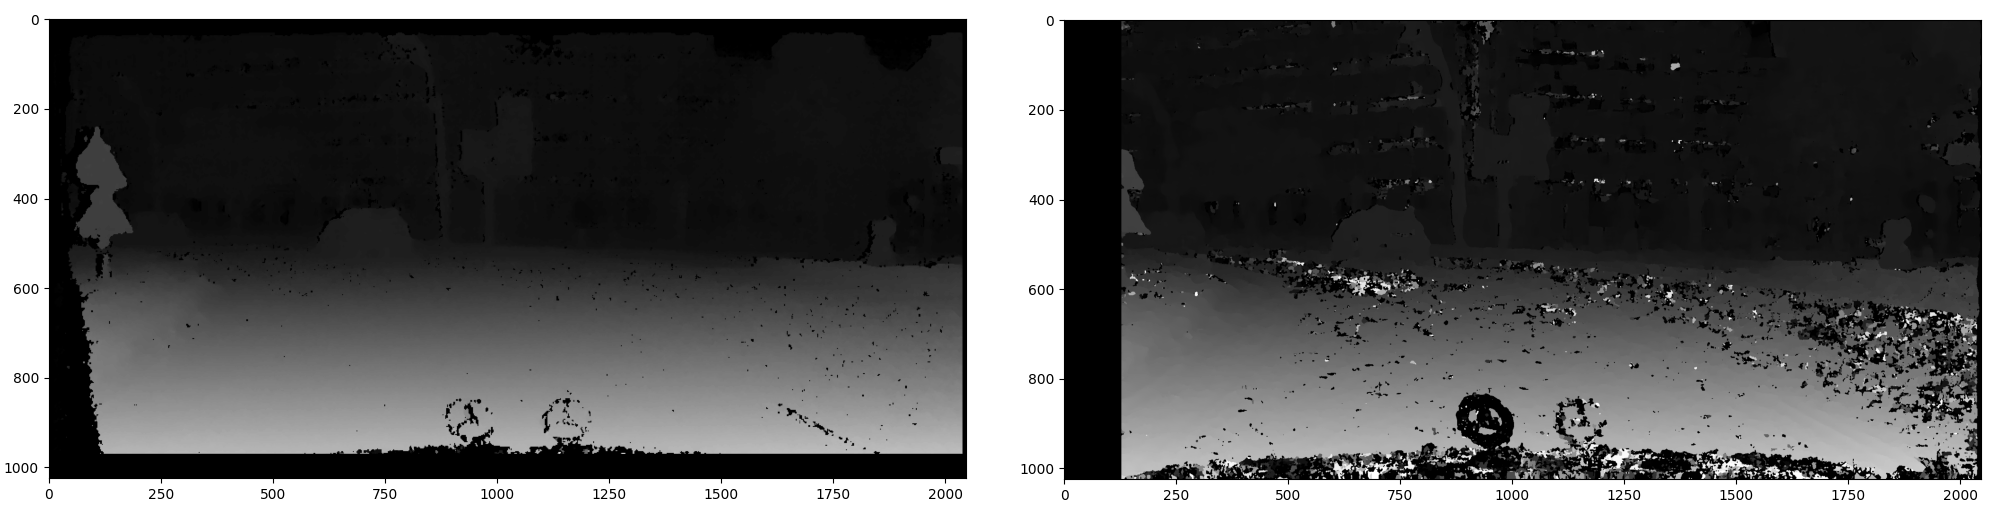
\includegraphics[width=\textwidth]{figures/disparity_1.png}}{disparity example}
\caption[Tämä on lyhyt kuvateksti.]{Vasemmalla tarjottu totuus. Oikealla opencv tulos stereo kuvasta.}
\label{fig:disparity1}
\end{figure}
    
Syvyysdatan kerääminen stereokuvista on mahdollista opencv2 kirjaston avulla.
Sumennus lisättiin jotta mahdolliset kameran aiheuttamat häiriöt saadaan minimoitua.
Käytetyt parametrit tarkoittavat että mahdollisia disparity tasoja on 128 ja alue jolta samankaltaisuutta verrataan on 20 pikselin kokoinen.
Funktiota ajettin HH modessa, joka tarkoittaa että se suoritetaan algoritmin alkuperäisellä suoritustavalla, 
eikä kevennetyllä jota käytetään muistin säästämiseksi.

Tuloksestamme huomaamme häiriötä jota totuudessa ei ole.
Tämä johtuu todennäköisesti kohdista kuvista joista Hirschmullerin-algoritmi ei pysty tunnistamaan vastaavaa kohtaa toisessa kuvassa.
Tämä voi tapahtua esimerkiksi asfaltin pinnassa jossa on hyvin samankaltaista tai varjoisilla alueilla. 

Tässä tilanteessa voisimme myös kouluttaa verkon jonka avulla saisimme hankittua syvyysdata,
mutta koska syvyysdata ei ole yleisesti saatavilla olevaa koulutusdataa,
ei voida olettaa että se olisi saatavilla tulevissa toteutuksissa. 

\subsection{Semanttinen Segmentointi}

Aineistossa on jo olemassa totuus segmentaatiodatasta.
Käytämme tätä valmista dataa, mutta koulutamme silti sitä varten myös uuden verkon.
Koulutettu verkko on hyvin yksinkertainen ja käyttää valmiita pytorch komponentteja.
Data on koulutettu\ fcn\_resnet50 avulla \cite{pytorchfcnresnet50}, ilman esikoulutettuja painoja. Optimointiin on käytetty Adam-algoritmia ja häviöfunktioksi on valittu CrossEntropyLoss-funktio.
Datasetin mallia on yksinkertaistettu tarpeen mukaan: kaikki liikkuvat kohteet, kuten autot ja ihmiset, on yhdistetty yhdeksi luokaksi ja kaikki muu toiseksi luokaksi.
Näin saadaan yksinkertaisempi malli, jonka avulla voidaan kuvasta tunnistaa kaikki liikkuvat kohteet Kuva \ref{fig:segmentation1}.

\begin{figure}[h]
\centering
\pdftooltip{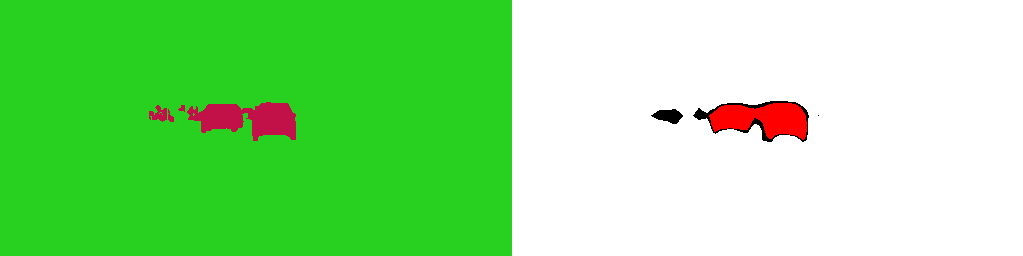
\includegraphics[width=\textwidth]{figures/segmentation1.png}}{segmentation example}
\caption[Tämä on lyhyt kuvateksti.]{Vasemmalla tarjottu totuus. Oikealla mallin tuottama.}
\label{fig:segmentation1}
\end{figure}
    

Tällä tavalla tehty malli antaa meille riittäviä tuloksia alkuperäiseen totuuteen verrattuna.
Ja sen kouluttaminen on myös melko yksinkertaista.
Tätä mallia ei kuitenkaan tarvita kuin lopullisen mallin luomiseen mahdollisissa muissa käyttökohteissa, joissa dataa ei ole saatavilla.
Voi kuitenkin olla helpompaa segmentoinnin sijaan, arvioida suoraan asioiden alla oleva syvyys.
Kuitenkin jos data tuotetaan esimerkiksi useilla kuvilla samoista kohdista joissa kohteet liikkuvat,
on segmentaatio mallista enemmän hyötyä.
Koska sitä voisi tälläisissä tapauksissa käyttää pelkästään taustasyvyys arvioinnin tuottamiseen, ilman syvyyksien arvaamista.

\section{Datan muodostus}

Niin kuin aikaisemmin jo mainittu, tavoite on jalostaa data muotoon, jossa kaikki liikkuvat kohteet on hävitetty syvyysdatasta.
Koska käytetty data on kaupunkidataa, tämä tarkoittaa autojen sekä ihmisten poistamista kuvista.
Koska käytettävissämme on kuvien segmentaatiodata, voidaan niiden alue poistamalla dispariteetista saavuttaa tila, jossa niitä ei oteta huomioon.

Kun liikkuvien objektien alue on poistettu, pitää niiden alla oleva alue generoida jotenkin. 
Kyseisten alueiden alla voi olla miltei mitä tahansa, 
ja ei ole selkeää ja helppoa keinoa sitä tietää. 
Alueen alle voi jäädä taloja joissa on erikoisia kulmia, puita, pensaita postilaatikoita tolppia ja mitä tahansa muuta. 
Tästä johtuen ei voida olettaa, että kyseinen malli olisi erityisen tarkka.
Kuitenkin alueen karkeaan arviointiin tuotetun datasetin pitäisi olla riittävä.
On tärkeä muistaa, että huonosti toteutettu dataset tuottaa myös huonoja tuloksia tuottavan mallin.

Tässä työssä mallin käsittelyä yritettiin vertikaalisella ja horisontaalisella pyyhkäisyllä, sekä niiden yhteistuloksella.
Tämä tarkoittaa että jokainen yhtenäinen alue etsittiin ja niiden syvyysarvot otettiin niiden reunoilta,
ja pyyhkäistiin läpi täsmäämään vastakkaisen reunan arvoon.
Tämä tarkoittaa, että jos kohteen takana on esimerkiksi puu vertikaalinen pyyhkäisy osaisi ottaa sen huomioon.
Jos kohteen takana sen sijaan on aita vertikaalien pyyhkäisy osaisi ottaa sen huomioon.
Ja yhdistetyssä tavassa nämä arvot on summattu, joten sen pitäisi olla keskiarvoltaan hyvä. 

\begin{figure}[h]
\centering
\pdftooltip{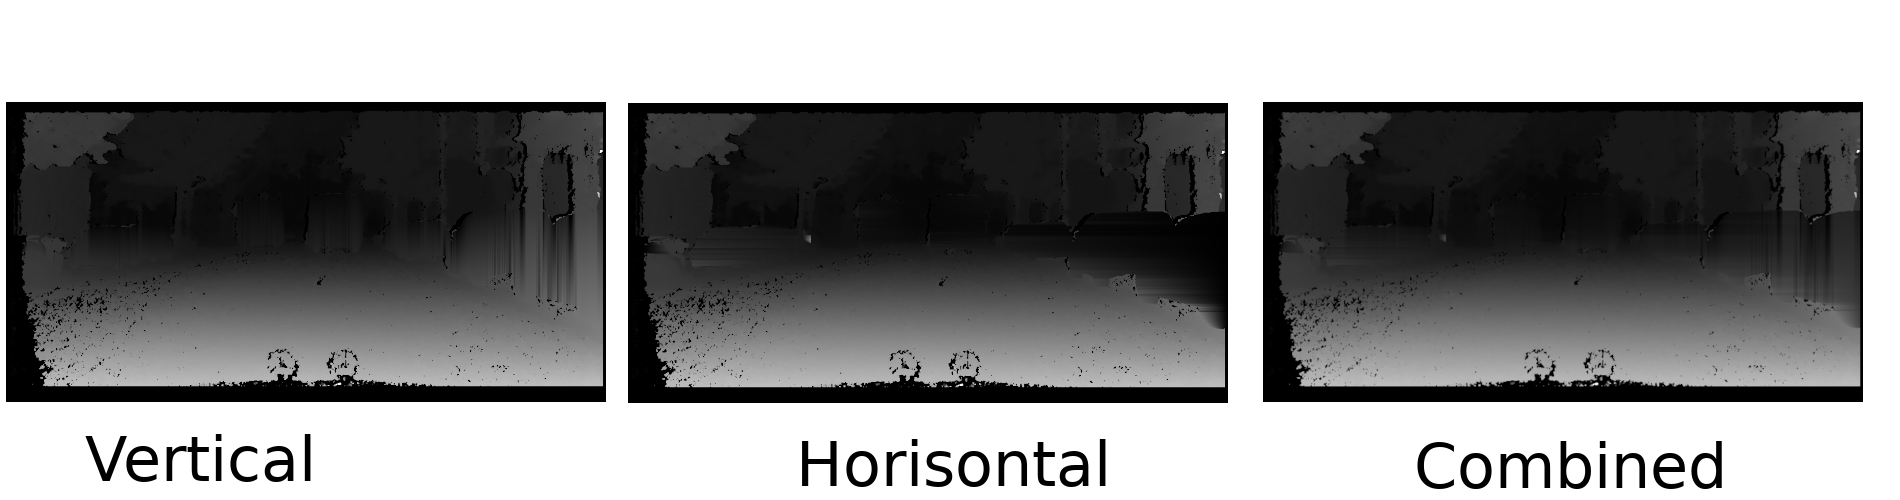
\includegraphics[width=\textwidth]{figures/swipe.png}}{Swipe}
\caption{Eri tyypin pyyhkäisyt syvyyden arviointiin}
\label{fig:swipe}
\end{figure}


Tässä kuvassa Kuva \ref{fig:swipe} on esitelty tavat vertikaali horisontaali sekä niiden yhdistetty arvo. 
Siitä huomataan että mikään tavoista ei ole täydellinen.
Tästä johtuen jotta datasta saadaan edes jollain tavalla käytettävää, tulee se käydä ensin läpi. 

Kuvien manuaalisessa valinnassa vertailtiin yllä mainittujen kuvien lisäksi pyyhkäisyjä,
jotka ylittävät tunnistetun reunan 50:llä pikselillä.
Datan läpikäynnin jälkeen valituksi tuli seuraavanlaisia kuvia.

\begin{figure}[h]
\centering
\pdftooltip{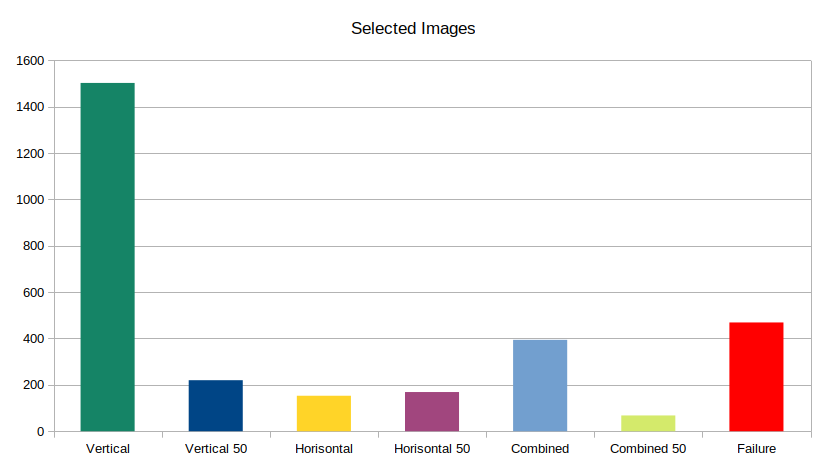
\includegraphics[width=\textwidth]{figures/selectedimages.png}}{Selected}
\caption{Selected}
\label{fig:selected}
\end{figure}

Tästä huomaamme että vertikaalinen valinta oli yleisin Kuva \ref{fig:selected} .
Yleensä jos horisontaalista dataa tarvittiin, se yleensä kannatti yhdistää vertikaalidataan.
Tämä johtuu todennäköisesti datan luonteesta. Suuri osa kohteista on melko lähellä kameraa ja reunassa.
Tämä johtaa tilanteeseen jossa analysoitavan alueen oikealla tai vasemmalla puolella ei ole tarpeeksi syvyysdataa jota voisi käyttää syvyyden generoimiseen.
Vertikaalipyyhkäistyjen kuvien data on myös todennäköisemmin oikein, koska suurin osa datasta on tieltä joka jatkuu eteenpäin.
Näin ollen ylempänä kuvassa kauempana oleva tasainen pyyhkäisy on todennäköisemmin oikein, kuin vasemmalta oikealle tuleva, joka tuo tulokseen enemmän satunnaisuutta.
Näin ollen koska kuvat on käsin silmämääräisesti valittuja, luonnollisimman näköiset kuvat ovat todennäköisesti valittuja.
Yhden kuvan valitsemiseen ei kuitenkaan ole käytetty paljoa aikaa vaan se on hyvin ”fiilis pohjaista”.

Yleisimmät asiat mitkä toivat ongelmia, olivat segmentoitujen alueiden vieressä olevat epäselvyydet.
Sekä alueet jotka olivat niin reunassa että niiden vierest käytettävän syvyyden saanti ei ollut mahdollista.
Jatkokehityksessä näitä ongelmia voisi yrittää parantaa muutamilla tavoilla. 

Tunnistettuja alueita laajentamalla voisimme onnistua piilottamaan joitan tunnistettujen alueiden reunoilla esiintyviä syvyysdatan häiriöitä.
Koska emme ole kiinnostuneita tunnistamaan asioita vaan piilottamaan ne, ei kovin suuri tarkkuus ole tarpeellista.
Jälkianalysoinnin kannalta myöskin liian suuri alue on huomattavasti pienempi harmi kuin liian pieni alue.

Tulosta voisi myös parantaa siistimällä disparitaatiodatasta kohinaa suodattamalla.
Tämä todennäköisesti poistaisi jotain tärkeää dataa,
mutta jälleen kerran tavoiteltu tarkkuus ei ole niin suuri että tästä pitäisi koitua suuresti haittaa,
koska yleinen ongelma on, että dataa ei ole saatavilla kuvan ulkopuolelta.

Koulutsdatan kuville voitaisiin luoda syvyyttä arvioiva kehys.
Tämä varmistaisi että syvyys on aina saatavilla, 
ja tällaisen kehyksen generointi pitäisi olla mahdollista datan samankaltaisuudesta johtuen.

Yksi yleisesti ongelmia tuottava tunnistettu kohde ovat ihmiset.
Ihmiset ovat monimutkaisempia muotoja kuin autot.
Näin ollen myös mallissa, ihmisen erottelu on tarkempaa.
Kuitenkin joissain kuvissa,
jos ihminen peitetään pienimmän ja suurimman koordinaatin peittävällä kuutiolla,
menetetään paljon dataa jota, ihmisen ympäriltä on havaittavissa.
Tätä varten voisi olla hyöydyllistä kirjoittaa algoritmi joka arvioisi muutoksen alueella olevia suurimpia eroja,
ja ehkä suodattaa suurimmat muutokset pois. Näin menetettäisiin osa datasta,
mutta todennäköisesti myös suurimmat virheet saataisiin hävitettyä. 

Tällä tavalla tuotettu malli, vaatii paljon manuaalista työtä ja hyväksyntää.
Kuitenkin kun uusia malleja tehdään, ei niiden luomiseen ole oikoteitä.
Kuitenkin mitä enemmän tätä työtä tehdään,
sitä helpommaksi se olemassa olevan mallin avulla tulee.
Manuaalisesta työstä ei kuitenkaan koskaan pääse datan validoinnissa pois,
jos käytössä ei ole parempaa lähtödataa.
Jos datasetti muodostettaisiin ottamalla samasta kohdasta useita kuvia,
niin kauan että kaikki liikkuvat kohteet olisivat poistuneet,
voitaisiin sen ja segmentaatiomallin avulla luoda huomattavasti parempaa koulutusdataa. 

\section{Lopullinen malli}

Datasta koulutettiin malli samalla pytorchin tarjoamalla "fcn\_resnet50" \cite{pytorchfcnresnet50} neuroverkolla kuin segmentaatiovaiheessa.
Ulostulon muoto jaettiin 128 luokkaan, jotka vastaavat eri syvyyttä.
Sisääntulona annettiin 2 harmaata kuvaa 3-ulotteisen matriisin eri kerroksissa.
Näin voitiin käyttää valmista segmentaatio mallia värikuva sisääntulolla, kahden stereo-mustavalkokuvan analysointiin ja tuottaa sillä syvyyskartta.

\begin{figure}[h]
\centering
\pdftooltip{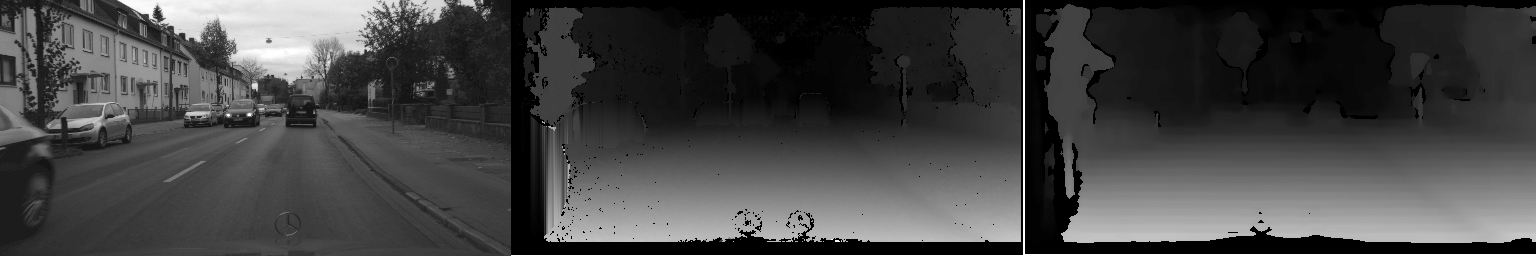
\includegraphics[width=\textwidth]{figures/model.png}}{Model}
\caption{Kuvassa vasemmalta oikealle; alkuperäinen kuva, rakennettu totuus, koulutetun mallin lopputulos.}
\label{fig:model}
\end{figure}



Kuvasta Kuva \ref{fig:model}  nähdään että, koulutus itsessään pystyy tuottamaan hyvin samankaltaisia kuvia kuin laskettu malli. Koulutettu malli kuitenkin oletetusti perii koulutusdatan heikkoudet. Koska käytetty automatisoitu tapa ei tuota täydellistä dataa, ei myöskään koulutettu malli ole täydellinen. 

Kuitenkin tässä tilanteessa, jossa ei ole tarvetta niin tarkalle lopputulokselle, tuottaa koulutettu malli vähemmän häiriötä kuin koneellisesti tuotettu malli. 